The behavior is described figure \ref{fig:behavior}.
A classical transaction starts with an order to established a communication with
an RBC. In this model we assume that the RBC belongs to the RBC accepting list.
Note that we have abstracted the different ways to contact an RBC (last known
number, number entered by the driver ...). Secondly, the MoRC sets up a safe radio
connection, then it initiates a radio communication with the RBC.
An order to terminate a radio communication session may occurred, in this case,
the MoRC sends a termination message to the RBC waits for the acknowledgment and
then releases the safe radio communication.
Our model does not manage the consistency of the successive order, we do not
impose any constraints to when the orders may occur. This may be done by external
tasks.

States \verb+INIT_COM+ and \verb+TERM_COM+ are decomposed as state automaton
handling the maximal number of try and the time out of requests.

Sate \verb+COM+ is decomposed as an automaton, it handles the lost of safe
radio.
\begin{figure}[htpb]
\centering
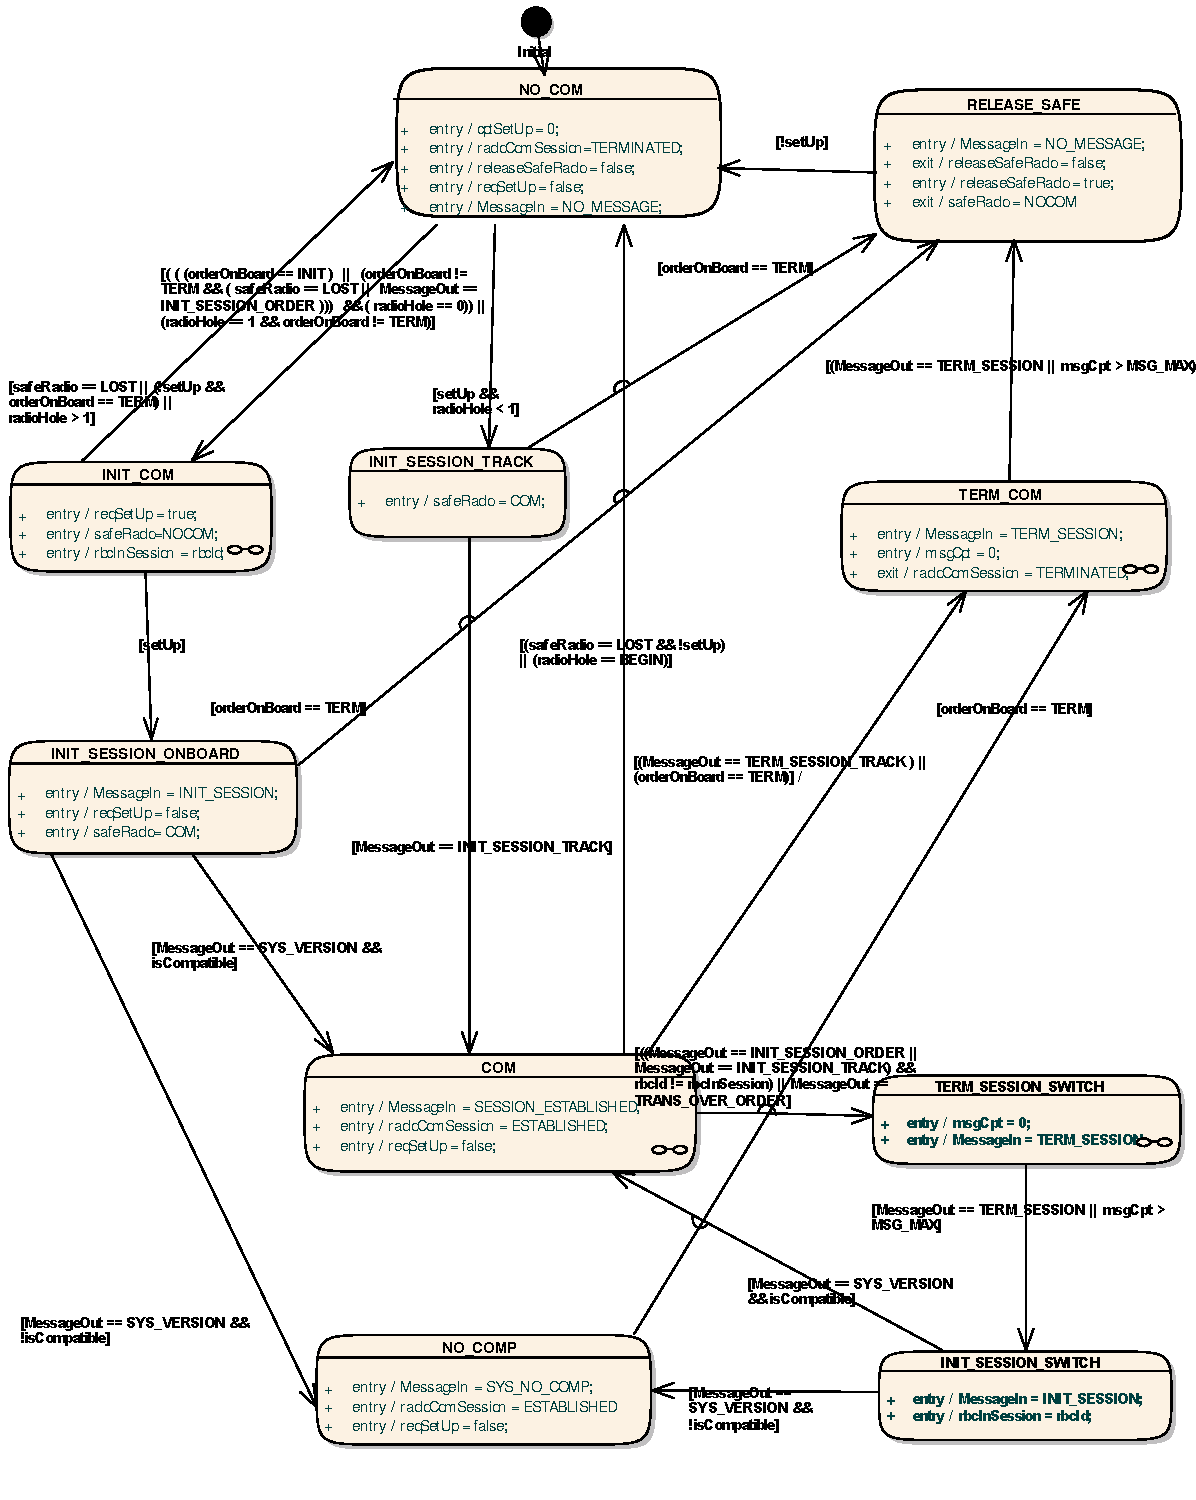
\includegraphics[width=\textwidth]{modelRadioManagment-T.pdf}
\caption{\label{fig:behavior}Automaton of the radio communication management}
\end{figure}

